% PART II — MATHEMATICAL & ALGORITHMIC FOUNDATIONS
\chapter{Chapter 2: Kinematics, Jacobian Control, Contact Mechanics, and Coulomb Friction}
\section{2.1 Forward Kinematics, Inverse Kinematics, and Jacobian Control}
A. Definition \& Purpose: Forward Kinematics (FK) maps joint coordinates q in R^7 into end-effector Cartesian pose x = FK(q) in SE(3) through homogeneous link transforms T\_0^1(q\_1)...T\_6^7(q\_7). Conversely, Inverse Kinematics (IK) determines joint increments dq achieving a desired Cartesian displacement dx, solving the problem of commanding intuitive 3D task goals [dx, dy, dz] with a 7-DOF arm.

B. Why Selected \& Mathematical Formulation: Rather than asking RL policies to directly regress 7 coupled joint torques (which requires orders of magnitude more exploration samples), this repository exposes compact 4D/5D task-space actions mapped via PyBullet's Damped Least-Squares (DLS) Jacobian pseudoinverse (Equation 1–2). The Jacobian J(q) in R^(6x7) relates joint velocities dq/dt to spatial twist dx/dt = J(q) dq/dt. Pure pseudoinverses J^T (J J^T)^(-1) explode near kinematic singularities where det(J J^T) -> 0; adding damping lambda = 0.05 stabilizes inversion while projecting neutral posture regularization (I - J\# J) k\_0 (q\_0 - q\_t) into the 1-DOF null space.

\begin{figure}[htbp]\centering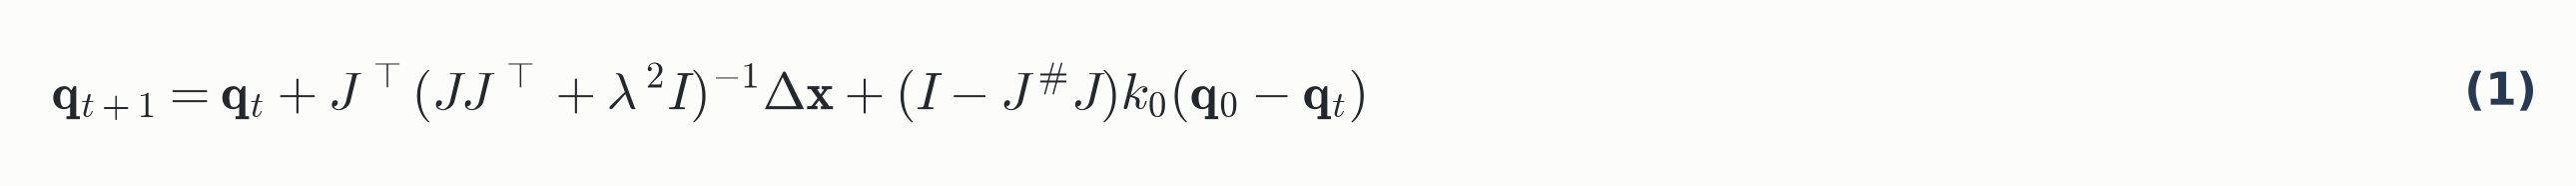
\includegraphics[width=0.9\linewidth]{../../assets/equations/eq_01.png}\caption{Equation (1): Damped Least-Squares Inverse Kinematics with null-space posture regularization.}\end{figure}
\begin{figure}[htbp]\centering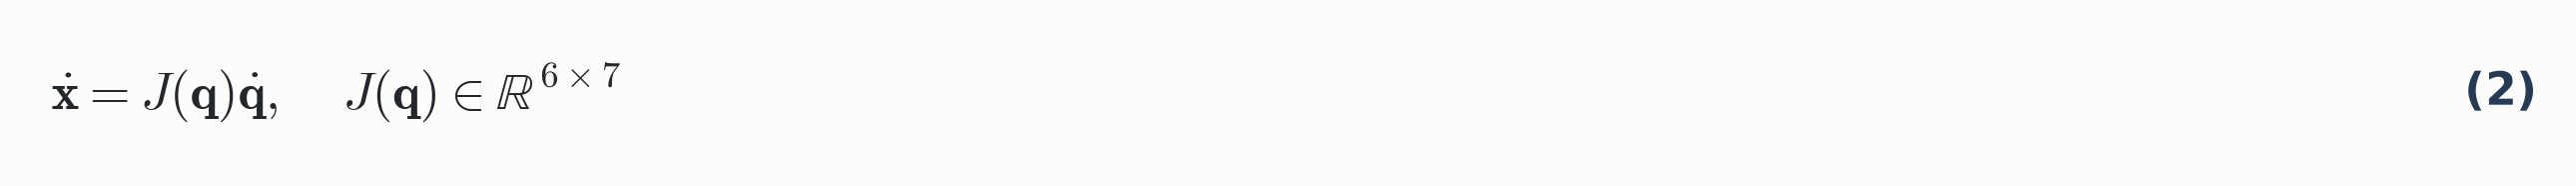
\includegraphics[width=0.9\linewidth]{../../assets/equations/eq_02.png}\caption{Equation (2): Instantaneous Jacobian velocity mapping for 7-DOF spatial twist.}\end{figure}
\begin{figure}[htbp]\centering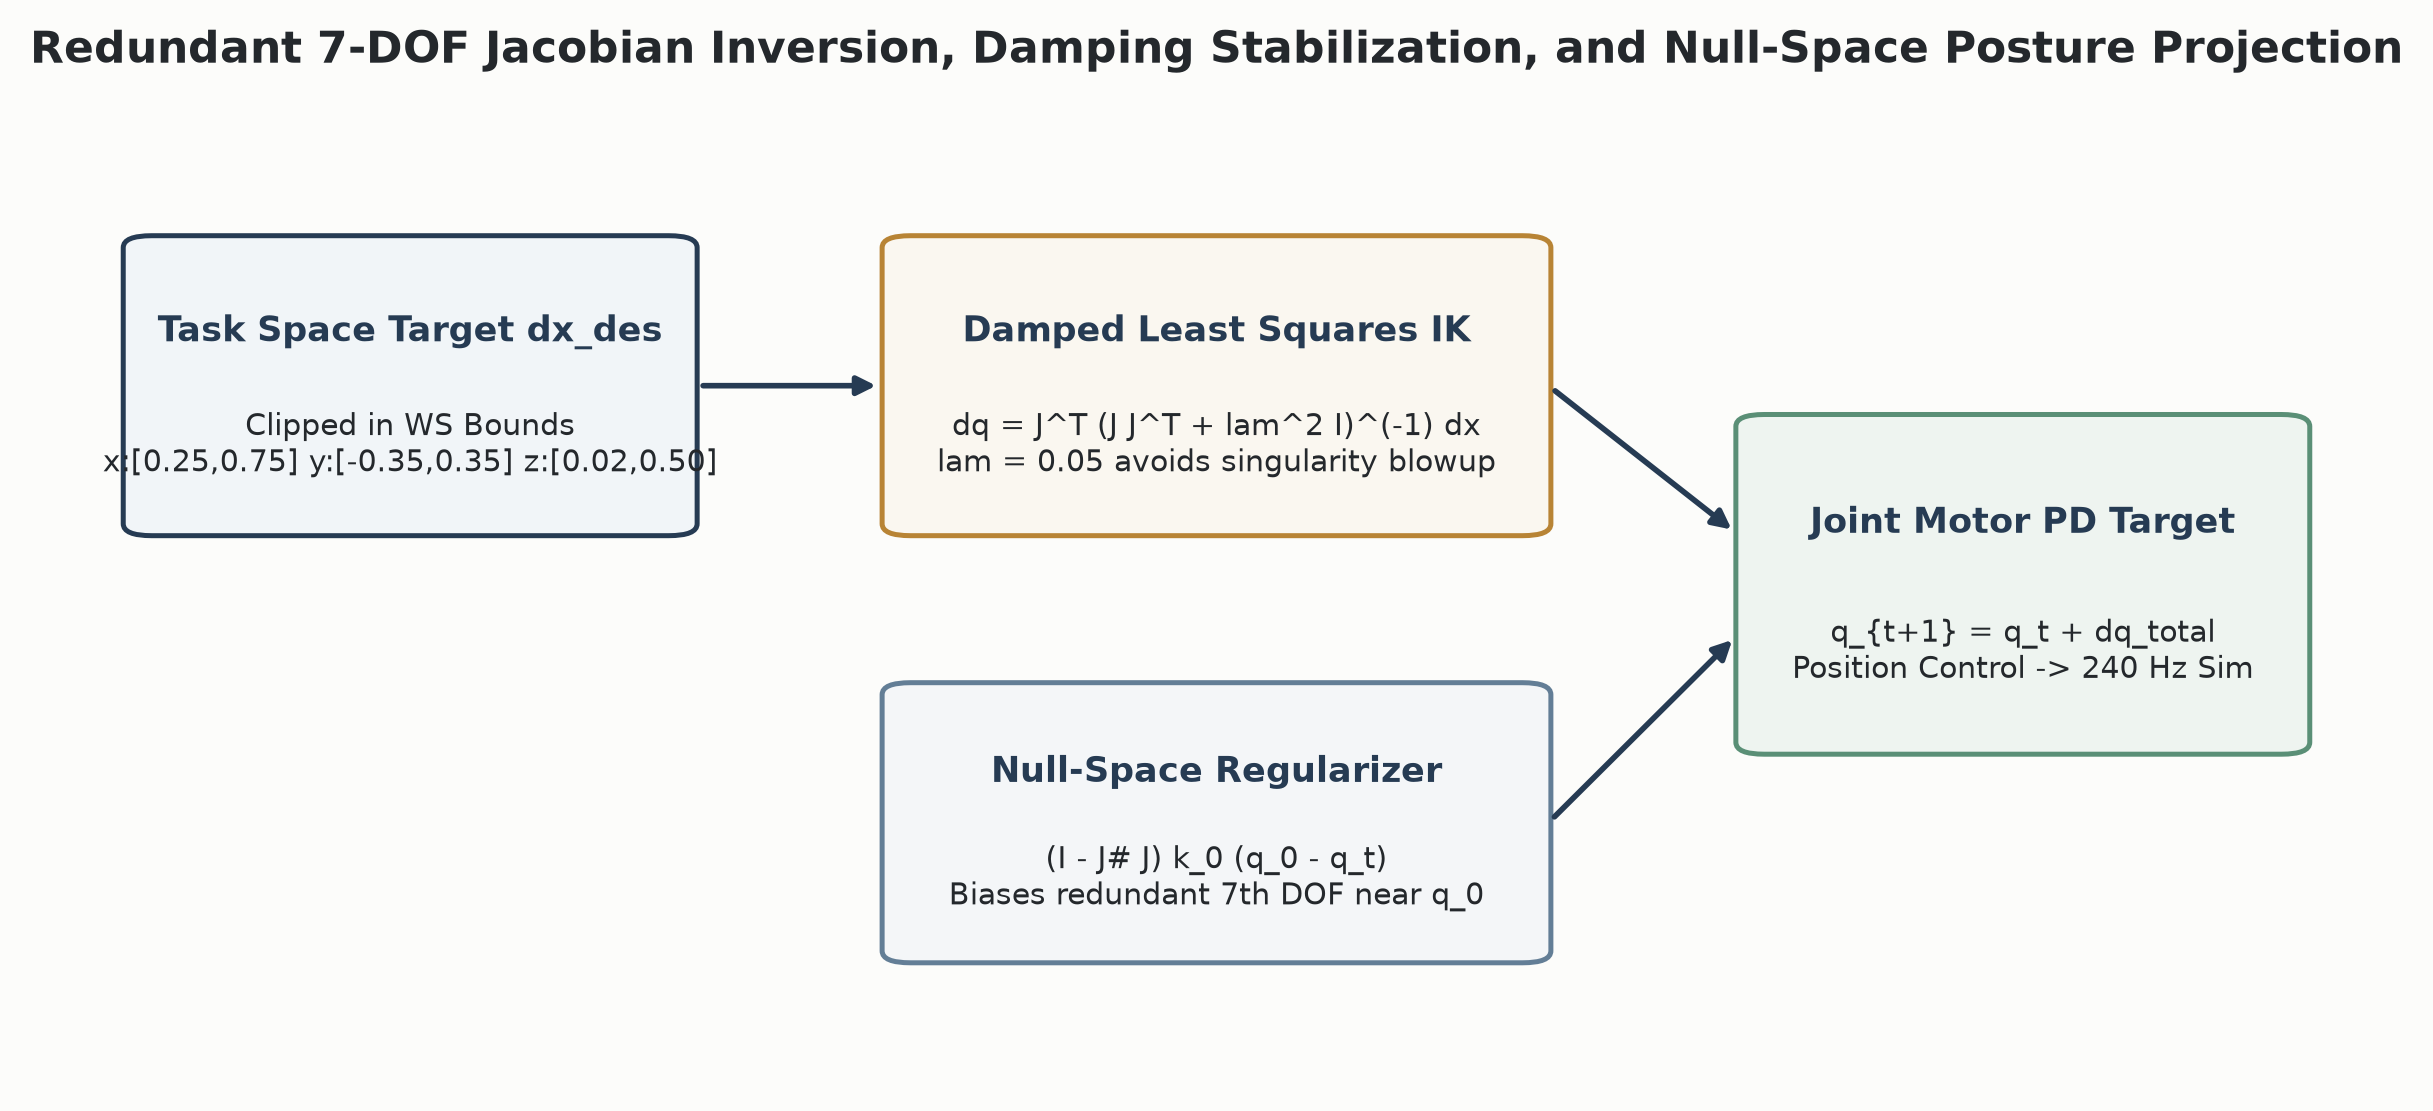
\includegraphics[width=0.9\linewidth]{../../assets/diagrams/diag_04_jacobian_and_control.png}\caption{Figure 2.1: Jacobian inversion, damping lambda=0.05 conditioning, and null-space posture regularization in FrankaPanda.calculate\_ik.}\end{figure}
\begin{lstlisting}[caption={src/robots/panda.py :: FrankaPanda.calculate\_ik \& clip\_to\_workspace}]
clipped_pos = self.clip_to_workspace(target_position)
all_ik_angles = p.calculateInverseKinematics(
    bodyUniqueId=self.body_id, endEffectorLinkIndex=self.ee_link_idx,
    targetPosition=list(clipped_pos), targetOrientation=orn,
    lowerLimits=self.joint_lower_limits, upperLimits=self.joint_upper_limits,
    jointRanges=self.joint_ranges, restPoses=self.neutral_joint_positions,
    maxNumIterations=100, residualThreshold=1e-4, physicsClientId=self.cid,
)
# Clips XYZ within ws_x=[0.25,0.75], ws_y=[-0.35,0.35], ws_z=[0.02,0.50]; solves DLS IK in <1ms.
\end{lstlisting}
C. Practical Example, Alternatives \& Real-World Context: In Phase 1, 5 validation waypoints confirmed 0.7 mm to 4.5 mm tracking accuracy. Alternatives include QP whole-body velocity controllers (OSQP) and operational-space torque control, which offer superior dynamic impact compliance at the cost of requiring accurate inertia matrices. In real manufacturing and surgical arms, damped Jacobian IK forms the universal inner kinematics layer beneath high-level planners.

\section{2.2 Contact Mechanics, Parallel-Jaw Grasping, and Coulomb Friction Cones}
A. Definition \& Internal Physics: Grasp stability during lifting is governed by unilateral normal squeeze forces F\_{n,9}, F\_{n,10} applied by Panda finger links 9 and 10 onto opposite cube faces, creating shear load capacity limited by Coulomb's friction cone |f\_s| <= mu * F\_n (Equation 9). To elevate an object of mass m under upward liftoff acceleration a\_z without slip, total bilateral squeeze force must obey F\_{n,req} >= m(g + a\_z) / (2 * mu).

\begin{figure}[htbp]\centering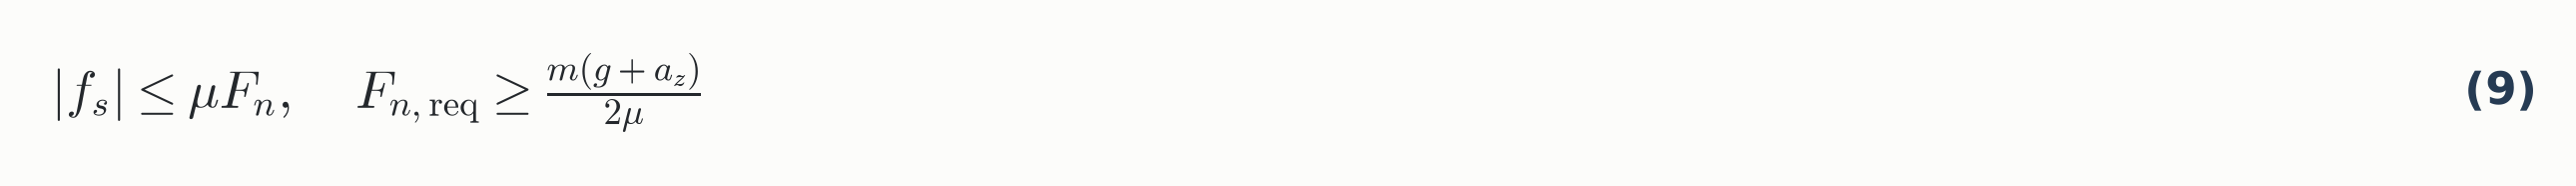
\includegraphics[width=0.9\linewidth]{../../assets/equations/eq_09.png}\caption{Equation (9): Coulomb friction cone limit and minimum normal squeeze force invariant.}\end{figure}
\begin{figure}[htbp]\centering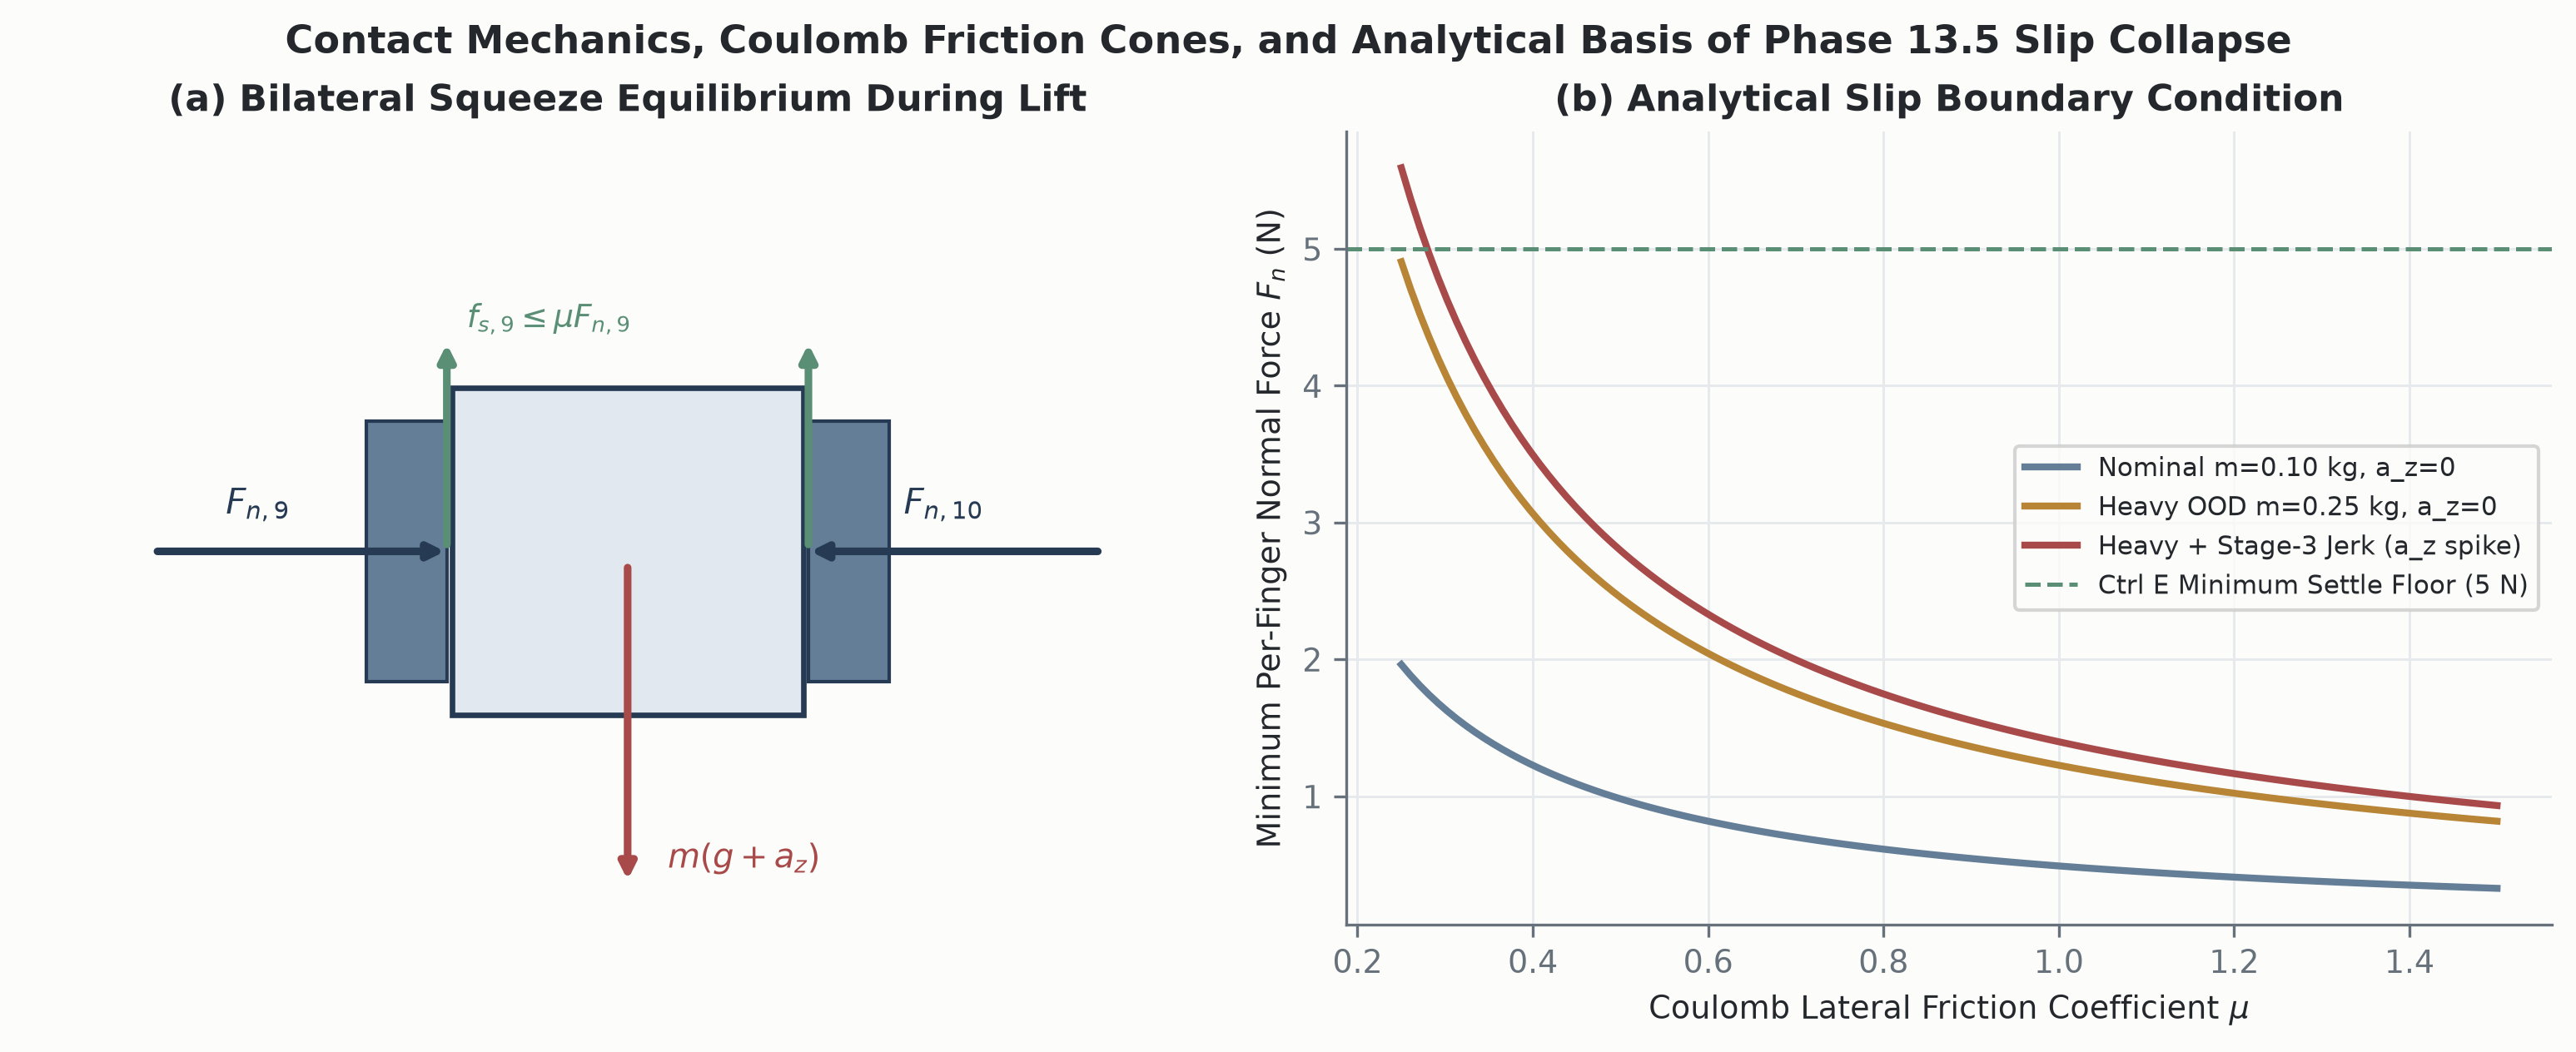
\includegraphics[width=0.9\linewidth]{../../assets/diagrams/diag_05_contact_and_friction_cones.png}\caption{Figure 2.2: (a) Bilateral gripper free-body force diagram; (b) Minimum required normal force across friction mu showing OOD slip cliff.}\end{figure}
\begin{figure}[htbp]\centering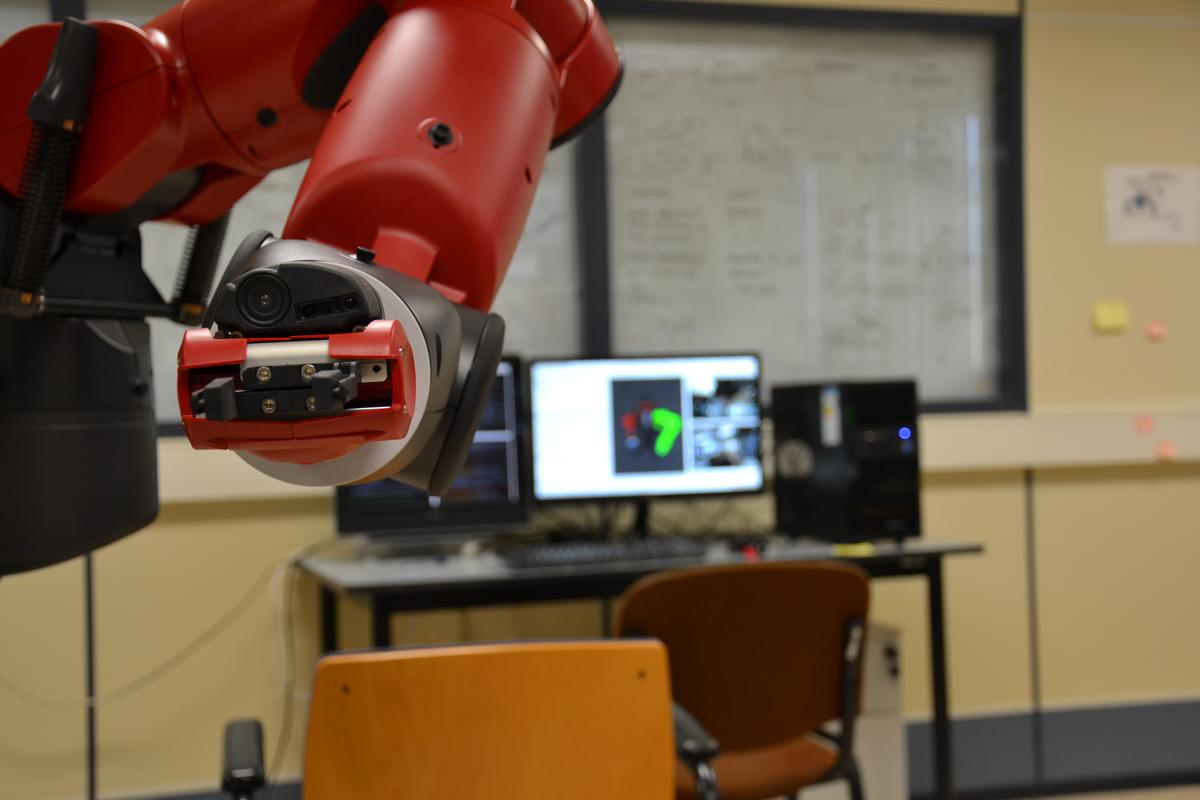
\includegraphics[width=0.9\linewidth]{../../assets/photographs/photo_01_parallel_gripper.jpg}\caption{Figure 2.3: Real-world parallel-jaw robotic gripper and wrist vision camera in a university research workstation. Source: Wikimedia Commons (File:Baxter\_robot's\_gripper.JPG), Author: Gustavo A. Casan, License: CC BY-SA 4.0.}\end{figure}
B. Evidence \& Project Lessons Learned: Two major failures traced directly back to Equation (9). First, in Phase 6 (ERR-001), default PyBullet finger friction could not hold a 0.10 kg cube; configuring lateralFriction=2.0 and spinningFriction=0.1 fixed scripted pick-and-place. Second, in Phase 13.5, heavy OOD cubes (0.25 kg) under low friction (mu=0.3) combined with an impulsive a\_z=0.14 m/s^2 liftoff jerk spiked normal force to 68.4 N before snapping contact to 0.0 N (30.5\% GRASP\_BUT\_NO\_LIFT failure rate), directly inspiring Phase 14 Controller E's 3-tick settle + lift-rate safety shield.
